\documentclass[tikz, border=5pt]{standalone}
\usepackage{tikz}
\usetikzlibrary{arrows.meta}

\begin{document}
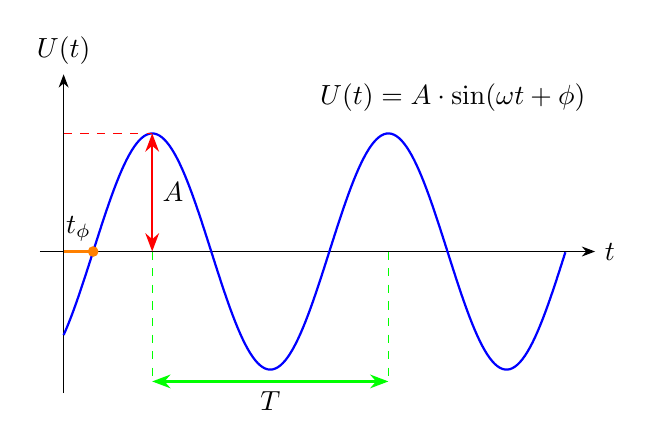
\begin{tikzpicture}[
    x=1.5cm, y=1.5cm,
    >=Stealth
]
    % Axes
    \draw[->] (-0.2,0) -- (4.5,0) node[right] {$t$}; 
    \draw[->] (0,-1.2) -- (0,1.5) node[above] {$U(t)$};

    % Sine wave
    \draw[blue, thick, domain=0:4.25, samples=200] plot (\x, {sin((\x-0.25)*180)});

    % Amplitude A
    \draw[dashed, red] (0,1) -- (0.75,1);
    \draw[<->, red, thick] (0.75,1) -- (0.75,0) node[midway, right, black] {$A$}; 

    % Phase shift phi
    \draw[orange, thick] (0, 0) -- (0.25, 0) node[midway, above, black] {$t_\phi$}; 
    \draw[orange, thick, fill] (0.25,0) circle (1.5pt);

    % Period T
    \draw[dashed, green] (0.75, 0) -- (0.75, -1.1);
    \draw[dashed, green] (2.75, 0) -- (2.75, -1.1);
    \draw[<->, green, thick] (0.75, -1.1) -- (2.75, -1.1) node[midway, below, black] {$T$}; 
    
    \node[anchor=north east, align=right] at (4.5, 1.5) {$U(t) = A \cdot \sin(\omega t + \phi)$};
\end{tikzpicture}
\end{document}
